% SPDX-License-Identifier: CC-BY-SA-4.0
%
% Copyright (C) 2026 embedded brains GmbH & Co. KG
\documentclass[tikz,border=4pt]{standalone}
\usepackage[T1]{fontenc}
\usepackage[scaled]{helvet}
\renewcommand{\familydefault}{\sfdefault}
\usetikzlibrary{arrows.meta,calc}
\definecolor{ebblue}{HTML}{1F4E79}
\definecolor{boxfill}{HTML}{EAF1F8}
\definecolor{codefill}{HTML}{FFF4E0}
\definecolor{codeline}{HTML}{9C6500}
\definecolor{groupfill}{HTML}{F5F5F5}
\definecolor{flow}{HTML}{404040}
\definecolor{earsfill}{HTML}{E8F4E8}
\definecolor{earsline}{HTML}{2E7D32}
\begin{document}
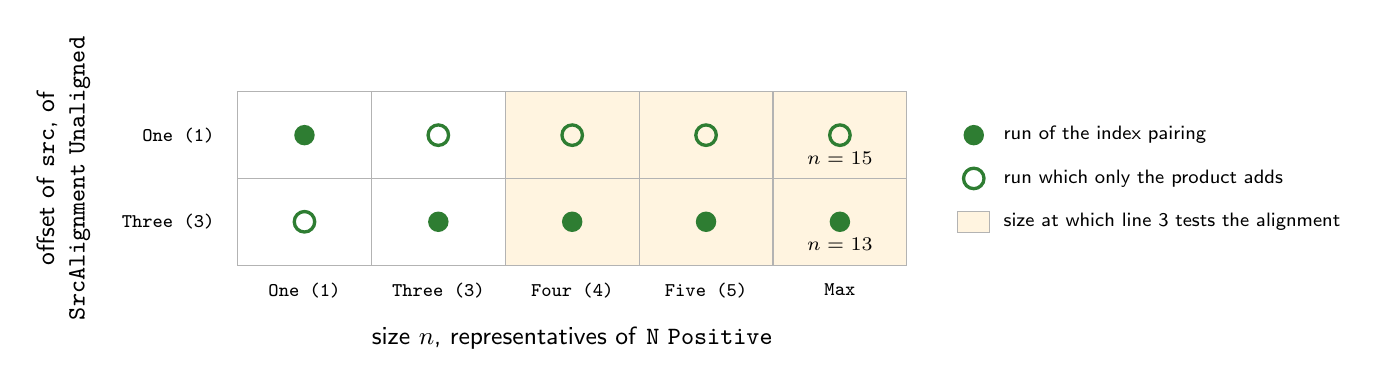
\begin{tikzpicture}[x=17mm, y=11mm, font=\small,
    cell/.style={draw=flow!40, fill=white},
    word/.style={draw=flow!40, fill=codefill},
    pair/.style={circle, fill=earsline, inner sep=0pt, minimum size=2.6mm},
    prod/.style={circle, draw=earsline, very thick, inner sep=0pt,
      minimum size=2.6mm},
    tick/.style={font=\scriptsize}]
  % The sizes of Positive against the offsets of Unaligned.
  \foreach \i in {0,...,4} {
    \foreach \j in {0,1} {
      \ifnum\i>1
        \draw[word] (\i-0.5, \j-0.5) rectangle (\i+0.5, \j+0.5);
      \else
        \draw[cell] (\i-0.5, \j-0.5) rectangle (\i+0.5, \j+0.5);
      \fi
    }
  }
  % The runs of the index pairing.
  \foreach \i/\j in {0/1, 1/0, 2/0, 3/0, 4/0} {
    \node[pair] at (\i, \j) {};
  }
  % The runs which only the product adds.
  \foreach \i/\j in {1/1, 2/1, 3/1, 4/1, 0/0} {
    \node[prod] at (\i, \j) {};
  }
  \node[tick, anchor=north] at (4, 0.92) {$n = 15$};
  \node[tick, anchor=north] at (4, -0.08) {$n = 13$};
  \foreach \j/\l in {1/One (1), 0/Three (3)} {
    \node[tick, anchor=east] at (-0.6, \j) {\texttt{\l}};
  }
  \foreach \i/\l in {0/One (1), 1/Three (3), 2/Four (4), 3/Five (5),
      4/Max} {
    \node[tick, below] at (\i, -0.6) {\texttt{\l}};
  }
  \node[below] at (2, -1.1) {size $n$, representatives of \texttt{N}
    \texttt{Positive}};
  \node[rotate=90, align=center] at (-1.8, 0.5)
    {offset of \texttt{src}, of\\\texttt{SrcAlignment} \texttt{Unaligned}};
  % The legend.
  \node[pair] (a) at (5.0, 1.0) {};
  \node[anchor=west, font=\scriptsize] at (5.15, 1.0)
    {run of the index pairing};
  \node[prod] (b) at (5.0, 0.5) {};
  \node[anchor=west, font=\scriptsize] at (5.15, 0.5)
    {run which only the product adds};
  \draw[word] (4.88, -0.12) rectangle (5.12, 0.12);
  \node[anchor=west, font=\scriptsize] at (5.15, 0.0)
    {size at which line 3 tests the alignment};
\end{tikzpicture}
\end{document}
